% Options for packages loaded elsewhere
\PassOptionsToPackage{unicode}{hyperref}
\PassOptionsToPackage{hyphens}{url}
\PassOptionsToPackage{dvipsnames,svgnames,x11names}{xcolor}
%
\documentclass[
  letterpaper,
  DIV=11,
  numbers=noendperiod]{scrartcl}

\usepackage{amsmath,amssymb}
\usepackage{lmodern}
\usepackage{iftex}
\ifPDFTeX
  \usepackage[T1]{fontenc}
  \usepackage[utf8]{inputenc}
  \usepackage{textcomp} % provide euro and other symbols
\else % if luatex or xetex
  \usepackage{unicode-math}
  \defaultfontfeatures{Scale=MatchLowercase}
  \defaultfontfeatures[\rmfamily]{Ligatures=TeX,Scale=1}
\fi
% Use upquote if available, for straight quotes in verbatim environments
\IfFileExists{upquote.sty}{\usepackage{upquote}}{}
\IfFileExists{microtype.sty}{% use microtype if available
  \usepackage[]{microtype}
  \UseMicrotypeSet[protrusion]{basicmath} % disable protrusion for tt fonts
}{}
\makeatletter
\@ifundefined{KOMAClassName}{% if non-KOMA class
  \IfFileExists{parskip.sty}{%
    \usepackage{parskip}
  }{% else
    \setlength{\parindent}{0pt}
    \setlength{\parskip}{6pt plus 2pt minus 1pt}}
}{% if KOMA class
  \KOMAoptions{parskip=half}}
\makeatother
\usepackage{xcolor}
\setlength{\emergencystretch}{3em} % prevent overfull lines
\setcounter{secnumdepth}{-\maxdimen} % remove section numbering
% Make \paragraph and \subparagraph free-standing
\ifx\paragraph\undefined\else
  \let\oldparagraph\paragraph
  \renewcommand{\paragraph}[1]{\oldparagraph{#1}\mbox{}}
\fi
\ifx\subparagraph\undefined\else
  \let\oldsubparagraph\subparagraph
  \renewcommand{\subparagraph}[1]{\oldsubparagraph{#1}\mbox{}}
\fi

\usepackage{color}
\usepackage{fancyvrb}
\newcommand{\VerbBar}{|}
\newcommand{\VERB}{\Verb[commandchars=\\\{\}]}
\DefineVerbatimEnvironment{Highlighting}{Verbatim}{commandchars=\\\{\}}
% Add ',fontsize=\small' for more characters per line
\usepackage{framed}
\definecolor{shadecolor}{RGB}{241,243,245}
\newenvironment{Shaded}{\begin{snugshade}}{\end{snugshade}}
\newcommand{\AlertTok}[1]{\textcolor[rgb]{0.68,0.00,0.00}{#1}}
\newcommand{\AnnotationTok}[1]{\textcolor[rgb]{0.37,0.37,0.37}{#1}}
\newcommand{\AttributeTok}[1]{\textcolor[rgb]{0.40,0.45,0.13}{#1}}
\newcommand{\BaseNTok}[1]{\textcolor[rgb]{0.68,0.00,0.00}{#1}}
\newcommand{\BuiltInTok}[1]{\textcolor[rgb]{0.00,0.23,0.31}{#1}}
\newcommand{\CharTok}[1]{\textcolor[rgb]{0.13,0.47,0.30}{#1}}
\newcommand{\CommentTok}[1]{\textcolor[rgb]{0.37,0.37,0.37}{#1}}
\newcommand{\CommentVarTok}[1]{\textcolor[rgb]{0.37,0.37,0.37}{\textit{#1}}}
\newcommand{\ConstantTok}[1]{\textcolor[rgb]{0.56,0.35,0.01}{#1}}
\newcommand{\ControlFlowTok}[1]{\textcolor[rgb]{0.00,0.23,0.31}{#1}}
\newcommand{\DataTypeTok}[1]{\textcolor[rgb]{0.68,0.00,0.00}{#1}}
\newcommand{\DecValTok}[1]{\textcolor[rgb]{0.68,0.00,0.00}{#1}}
\newcommand{\DocumentationTok}[1]{\textcolor[rgb]{0.37,0.37,0.37}{\textit{#1}}}
\newcommand{\ErrorTok}[1]{\textcolor[rgb]{0.68,0.00,0.00}{#1}}
\newcommand{\ExtensionTok}[1]{\textcolor[rgb]{0.00,0.23,0.31}{#1}}
\newcommand{\FloatTok}[1]{\textcolor[rgb]{0.68,0.00,0.00}{#1}}
\newcommand{\FunctionTok}[1]{\textcolor[rgb]{0.28,0.35,0.67}{#1}}
\newcommand{\ImportTok}[1]{\textcolor[rgb]{0.00,0.46,0.62}{#1}}
\newcommand{\InformationTok}[1]{\textcolor[rgb]{0.37,0.37,0.37}{#1}}
\newcommand{\KeywordTok}[1]{\textcolor[rgb]{0.00,0.23,0.31}{#1}}
\newcommand{\NormalTok}[1]{\textcolor[rgb]{0.00,0.23,0.31}{#1}}
\newcommand{\OperatorTok}[1]{\textcolor[rgb]{0.37,0.37,0.37}{#1}}
\newcommand{\OtherTok}[1]{\textcolor[rgb]{0.00,0.23,0.31}{#1}}
\newcommand{\PreprocessorTok}[1]{\textcolor[rgb]{0.68,0.00,0.00}{#1}}
\newcommand{\RegionMarkerTok}[1]{\textcolor[rgb]{0.00,0.23,0.31}{#1}}
\newcommand{\SpecialCharTok}[1]{\textcolor[rgb]{0.37,0.37,0.37}{#1}}
\newcommand{\SpecialStringTok}[1]{\textcolor[rgb]{0.13,0.47,0.30}{#1}}
\newcommand{\StringTok}[1]{\textcolor[rgb]{0.13,0.47,0.30}{#1}}
\newcommand{\VariableTok}[1]{\textcolor[rgb]{0.07,0.07,0.07}{#1}}
\newcommand{\VerbatimStringTok}[1]{\textcolor[rgb]{0.13,0.47,0.30}{#1}}
\newcommand{\WarningTok}[1]{\textcolor[rgb]{0.37,0.37,0.37}{\textit{#1}}}

\providecommand{\tightlist}{%
  \setlength{\itemsep}{0pt}\setlength{\parskip}{0pt}}\usepackage{longtable,booktabs,array}
\usepackage{calc} % for calculating minipage widths
% Correct order of tables after \paragraph or \subparagraph
\usepackage{etoolbox}
\makeatletter
\patchcmd\longtable{\par}{\if@noskipsec\mbox{}\fi\par}{}{}
\makeatother
% Allow footnotes in longtable head/foot
\IfFileExists{footnotehyper.sty}{\usepackage{footnotehyper}}{\usepackage{footnote}}
\makesavenoteenv{longtable}
\usepackage{graphicx}
\makeatletter
\def\maxwidth{\ifdim\Gin@nat@width>\linewidth\linewidth\else\Gin@nat@width\fi}
\def\maxheight{\ifdim\Gin@nat@height>\textheight\textheight\else\Gin@nat@height\fi}
\makeatother
% Scale images if necessary, so that they will not overflow the page
% margins by default, and it is still possible to overwrite the defaults
% using explicit options in \includegraphics[width, height, ...]{}
\setkeys{Gin}{width=\maxwidth,height=\maxheight,keepaspectratio}
% Set default figure placement to htbp
\makeatletter
\def\fps@figure{htbp}
\makeatother

\KOMAoption{captions}{tableheading}
\makeatletter
\makeatother
\makeatletter
\makeatother
\makeatletter
\@ifpackageloaded{caption}{}{\usepackage{caption}}
\AtBeginDocument{%
\ifdefined\contentsname
  \renewcommand*\contentsname{Table of contents}
\else
  \newcommand\contentsname{Table of contents}
\fi
\ifdefined\listfigurename
  \renewcommand*\listfigurename{List of Figures}
\else
  \newcommand\listfigurename{List of Figures}
\fi
\ifdefined\listtablename
  \renewcommand*\listtablename{List of Tables}
\else
  \newcommand\listtablename{List of Tables}
\fi
\ifdefined\figurename
  \renewcommand*\figurename{Figure}
\else
  \newcommand\figurename{Figure}
\fi
\ifdefined\tablename
  \renewcommand*\tablename{Table}
\else
  \newcommand\tablename{Table}
\fi
}
\@ifpackageloaded{float}{}{\usepackage{float}}
\floatstyle{ruled}
\@ifundefined{c@chapter}{\newfloat{codelisting}{h}{lop}}{\newfloat{codelisting}{h}{lop}[chapter]}
\floatname{codelisting}{Listing}
\newcommand*\listoflistings{\listof{codelisting}{List of Listings}}
\makeatother
\makeatletter
\@ifpackageloaded{caption}{}{\usepackage{caption}}
\@ifpackageloaded{subcaption}{}{\usepackage{subcaption}}
\makeatother
\makeatletter
\@ifpackageloaded{tcolorbox}{}{\usepackage[many]{tcolorbox}}
\makeatother
\makeatletter
\@ifundefined{shadecolor}{\definecolor{shadecolor}{rgb}{.97, .97, .97}}
\makeatother
\makeatletter
\makeatother
\ifLuaTeX
  \usepackage{selnolig}  % disable illegal ligatures
\fi
\IfFileExists{bookmark.sty}{\usepackage{bookmark}}{\usepackage{hyperref}}
\IfFileExists{xurl.sty}{\usepackage{xurl}}{} % add URL line breaks if available
\urlstyle{same} % disable monospaced font for URLs
\hypersetup{
  pdftitle={Robby - Homework 1},
  colorlinks=true,
  linkcolor={blue},
  filecolor={Maroon},
  citecolor={Blue},
  urlcolor={Blue},
  pdfcreator={LaTeX via pandoc}}

\title{Robby - Homework 1}
\author{}
\date{}

\begin{document}
\maketitle
\ifdefined\Shaded\renewenvironment{Shaded}{\begin{tcolorbox}[breakable, boxrule=0pt, sharp corners, frame hidden, enhanced, interior hidden, borderline west={3pt}{0pt}{shadecolor}]}{\end{tcolorbox}}\fi

\begin{Shaded}
\begin{Highlighting}[]
\FunctionTok{library}\NormalTok{(spatstat)}
\end{Highlighting}
\end{Shaded}

\begin{verbatim}
Loading required package: spatstat.data
\end{verbatim}

\begin{verbatim}
Loading required package: spatstat.geom
\end{verbatim}

\begin{verbatim}
spatstat.geom 3.2-5
\end{verbatim}

\begin{verbatim}
Loading required package: spatstat.random
\end{verbatim}

\begin{verbatim}
spatstat.random 3.1-6
\end{verbatim}

\begin{verbatim}
Loading required package: spatstat.explore
\end{verbatim}

\begin{verbatim}
Loading required package: nlme
\end{verbatim}

\begin{verbatim}
spatstat.explore 3.2-3
\end{verbatim}

\begin{verbatim}
Loading required package: spatstat.model
\end{verbatim}

\begin{verbatim}
Loading required package: rpart
\end{verbatim}

\begin{verbatim}
spatstat.model 3.2-6
\end{verbatim}

\begin{verbatim}
Loading required package: spatstat.linnet
\end{verbatim}

\begin{verbatim}
spatstat.linnet 3.1-1
\end{verbatim}

\begin{verbatim}

spatstat 3.0-6 
For an introduction to spatstat, type 'beginner' 
\end{verbatim}

\begin{Shaded}
\begin{Highlighting}[]
\FunctionTok{library}\NormalTok{(splancs)}
\end{Highlighting}
\end{Shaded}

\begin{verbatim}
Loading required package: sp
\end{verbatim}

\begin{verbatim}
The legacy packages maptools, rgdal, and rgeos, underpinning the sp package,
which was just loaded, will retire in October 2023.
Please refer to R-spatial evolution reports for details, especially
https://r-spatial.org/r/2023/05/15/evolution4.html.
It may be desirable to make the sf package available;
package maintainers should consider adding sf to Suggests:.
The sp package is now running under evolution status 2
     (status 2 uses the sf package in place of rgdal)
\end{verbatim}

\begin{verbatim}

Spatial Point Pattern Analysis Code in S-Plus
 
 Version 2 - Spatial and Space-Time analysis
\end{verbatim}

\begin{Shaded}
\begin{Highlighting}[]
\FunctionTok{library}\NormalTok{(spatial)}
\end{Highlighting}
\end{Shaded}

\begin{verbatim}

Attaching package: 'spatial'
\end{verbatim}

\begin{verbatim}
The following object is masked from 'package:spatstat.model':

    Strauss
\end{verbatim}

\hypertarget{point-process-homework-basics}{%
\section{Point Process Homework
(Basics)}\label{point-process-homework-basics}}

\hypertarget{problem-1}{%
\subsection{Problem 1}\label{problem-1}}

What are the two components needed to define a spatial point process?

\begin{quote}
\begin{enumerate}
\def\labelenumi{\arabic{enumi}.}
\tightlist
\item
  Event Locations (where and event did occur)
\item
  Event Space (where an event could occur)
\end{enumerate}
\end{quote}

\hypertarget{problem-2}{%
\subsection{Problem 2}\label{problem-2}}

What are the main components that define a homogeneous Poisson point
process?

\begin{quote}
\begin{enumerate}
\def\labelenumi{\arabic{enumi}.}
\tightlist
\item
  Stationarity and a constant intensity parameter Lambda
\item
  Complete Spatial Randomness (events are uniformly distributed over the
  study region)
\end{enumerate}
\end{quote}

\hypertarget{problem-3}{%
\subsection{Problem 3}\label{problem-3}}

What is the main difference between a homogeneous and heterogeneous
point process (pp)?

\begin{quote}
The main difference between the two point processes is that the
intensity of events within the study region is constant for the
homogeneous pp and not constant for the heterogeneous pp.
\end{quote}

\hypertarget{problem-4}{%
\subsection{Problem 4}\label{problem-4}}

Describe the differences between a regular, clustered, and homogeneous
(CSR) Poisson pp?

\begin{quote}
One can think of the relationship (and the difference between these
point patterns) as a spectrum ranging from a regular distribution of
points wherein no clustering is observed, moving to CSR in which each
event location is uniformly distributed and independent of each other
event location, and finally on the other end of the spectrum is
clustering, in which event locations are grouped up more than would be
random.
\end{quote}

\hypertarget{problem-5}{%
\subsection{Problem 5}\label{problem-5}}

For this problem, I was able to create a plot for each realization using
code from Dr.~French's github repo.

\hypertarget{regular-point-process}{%
\subsubsection{Regular Point Process}\label{regular-point-process}}

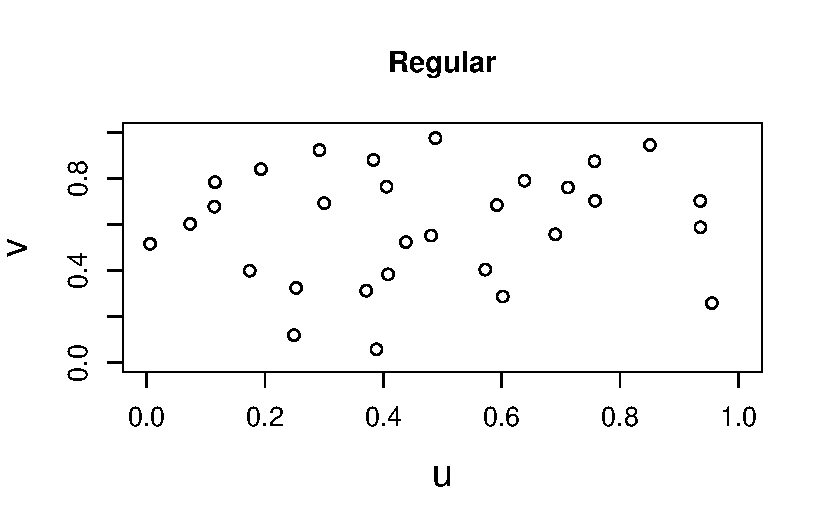
\includegraphics{robby_homework1_files/figure-pdf/unnamed-chunk-2-1.pdf}

\hypertarget{clustered-point-process}{%
\subsubsection{Clustered Point Process}\label{clustered-point-process}}

\begin{Shaded}
\begin{Highlighting}[]
\CommentTok{\# domain is unit square}
\NormalTok{domain }\OtherTok{=} \FunctionTok{cbind}\NormalTok{(}\FunctionTok{c}\NormalTok{(}\DecValTok{0}\NormalTok{,}\DecValTok{0}\NormalTok{,}\DecValTok{1}\NormalTok{,}\DecValTok{1}\NormalTok{), }\FunctionTok{c}\NormalTok{(}\DecValTok{0}\NormalTok{,}\DecValTok{1}\NormalTok{,}\DecValTok{1}\NormalTok{,}\DecValTok{0}\NormalTok{))}


\NormalTok{test }\OtherTok{\textless{}{-}} \FunctionTok{pcp.sim}\NormalTok{(}\AttributeTok{rho =} \DecValTok{5}\NormalTok{, }\AttributeTok{m =} \DecValTok{25}\NormalTok{, }\AttributeTok{s2 =} \FloatTok{0.01}\NormalTok{, }\AttributeTok{region.poly =}\NormalTok{ domain)}
\FunctionTok{plot}\NormalTok{(test, }\AttributeTok{xlim =} \DecValTok{0}\SpecialCharTok{:}\DecValTok{1}\NormalTok{, }\AttributeTok{ylim =} \DecValTok{0}\SpecialCharTok{:}\DecValTok{1}\NormalTok{, }\AttributeTok{xlab =} \StringTok{"u"}\NormalTok{, }\AttributeTok{ylab =} \StringTok{"v"}\NormalTok{, }
     \AttributeTok{cex.lab =} \FloatTok{1.5}\NormalTok{, }\AttributeTok{cex.axis =} \FloatTok{1.1}\NormalTok{)}
\FunctionTok{title}\NormalTok{(}\StringTok{"Clustered"}\NormalTok{)}
\end{Highlighting}
\end{Shaded}

\begin{figure}[H]

{\centering 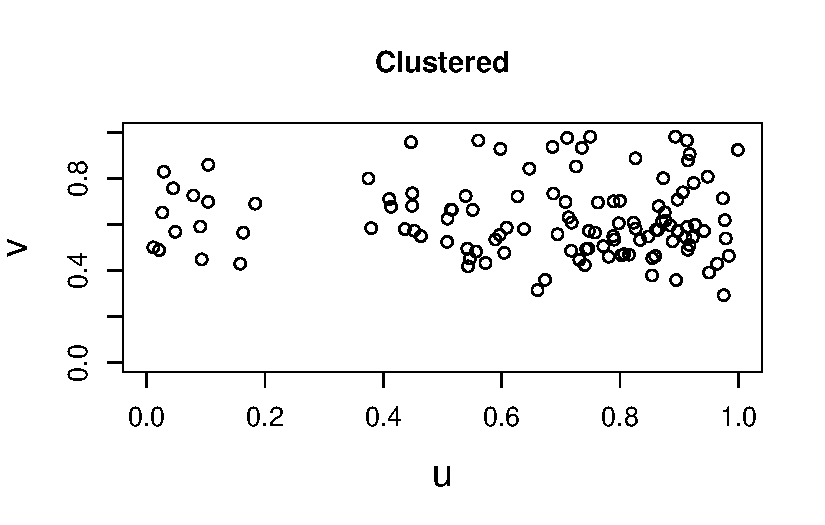
\includegraphics{robby_homework1_files/figure-pdf/unnamed-chunk-3-1.pdf}

}

\end{figure}

\hypertarget{csr-poisson-point-process}{%
\subsubsection{CSR Poisson Point
Process}\label{csr-poisson-point-process}}

\begin{Shaded}
\begin{Highlighting}[]
\FunctionTok{library}\NormalTok{(spatstat)}

\NormalTok{poi }\OtherTok{\textless{}{-}} \FunctionTok{rpoispp}\NormalTok{(}\DecValTok{50}\NormalTok{)}
\FunctionTok{plot}\NormalTok{(poi}\SpecialCharTok{$}\NormalTok{x,poi}\SpecialCharTok{$}\NormalTok{y,}\AttributeTok{xlab =} \StringTok{"u"}\NormalTok{, }\AttributeTok{ylab =} \StringTok{"v"}\NormalTok{, }\AttributeTok{main=}\StringTok{"Homogenous Poisson Point Process"}\NormalTok{)}
\end{Highlighting}
\end{Shaded}

\begin{figure}[H]

{\centering 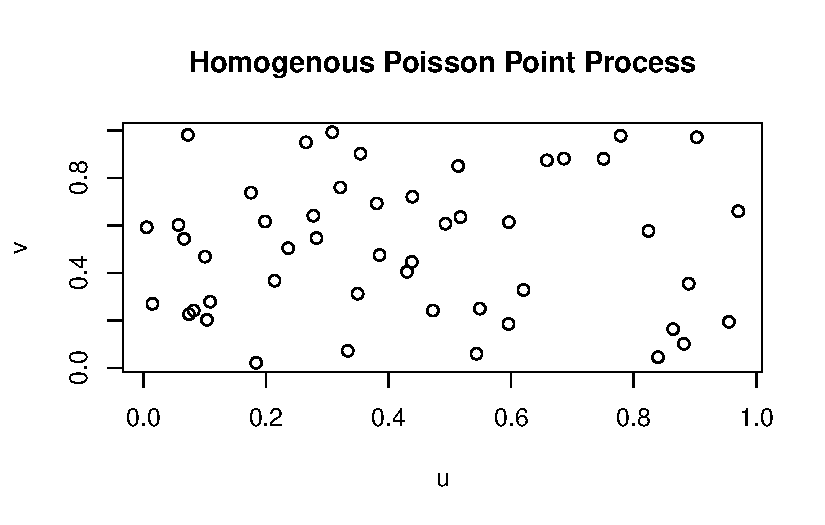
\includegraphics{robby_homework1_files/figure-pdf/unnamed-chunk-4-1.pdf}

}

\end{figure}

\hypertarget{problem-6}{%
\subsection{Problem 6}\label{problem-6}}

\begin{Shaded}
\begin{Highlighting}[]
\NormalTok{h1 }\OtherTok{\textless{}{-}} \FunctionTok{rpoispp}\NormalTok{(}\DecValTok{50}\NormalTok{)}

\FunctionTok{plot}\NormalTok{(h1}\SpecialCharTok{$}\NormalTok{x,h1}\SpecialCharTok{$}\NormalTok{y, }\AttributeTok{xlab =} \StringTok{"u"}\NormalTok{, }\AttributeTok{ylab =} \StringTok{"v"}\NormalTok{,}\AttributeTok{main=}\StringTok{"Poisson Point Process"}\NormalTok{)}
\end{Highlighting}
\end{Shaded}

\begin{figure}[H]

{\centering 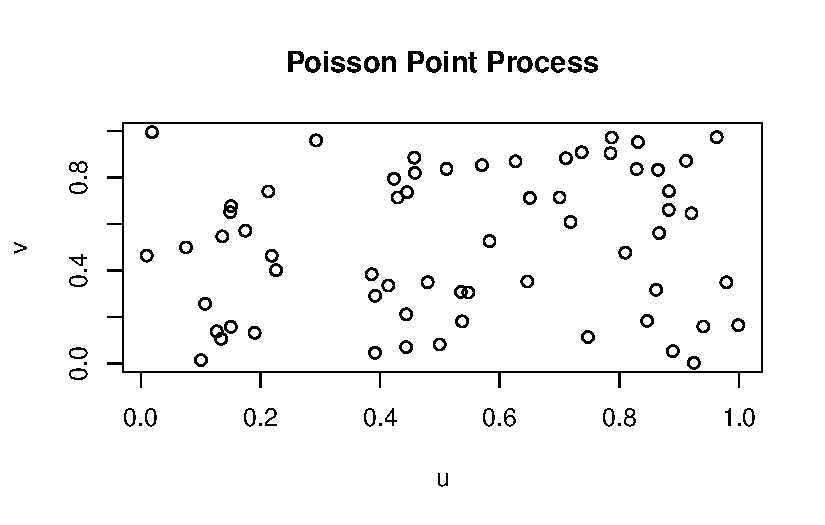
\includegraphics{robby_homework1_files/figure-pdf/unnamed-chunk-5-1.pdf}

}

\end{figure}

\begin{Shaded}
\begin{Highlighting}[]
\NormalTok{point\_count }\OtherTok{=} \FunctionTok{length}\NormalTok{(h1}\SpecialCharTok{$}\NormalTok{x)}
\FunctionTok{print}\NormalTok{(}\StringTok{"Total Points Generated: "}\NormalTok{)}
\end{Highlighting}
\end{Shaded}

\begin{verbatim}
[1] "Total Points Generated: "
\end{verbatim}

\begin{Shaded}
\begin{Highlighting}[]
\FunctionTok{print}\NormalTok{(point\_count)}
\end{Highlighting}
\end{Shaded}

\begin{verbatim}
[1] 63
\end{verbatim}

\begin{quote}
The h1 plot shows a seemingly random realization of 63 points. While
there is little evidence of overlapping event locations, we can see at
least one such pair of events which means this is not a regular plot,
and not indicative of clustering. Therefore, it seems the h1 plot could
be compatible with CSR.
\end{quote}

\hypertarget{problem-7}{%
\subsection{Problem 7}\label{problem-7}}

\begin{Shaded}
\begin{Highlighting}[]
\NormalTok{rcsr }\OtherTok{\textless{}{-}} \ControlFlowTok{function}\NormalTok{(lambda)\{}
\NormalTok{  region }\OtherTok{=} \FunctionTok{cbind}\NormalTok{(}\FunctionTok{c}\NormalTok{(}\DecValTok{1}\NormalTok{,}\DecValTok{0}\NormalTok{,}\DecValTok{0}\NormalTok{,}\DecValTok{1}\NormalTok{), }\FunctionTok{c}\NormalTok{(}\DecValTok{1}\NormalTok{,}\DecValTok{1}\NormalTok{,}\DecValTok{0}\NormalTok{,}\DecValTok{0}\NormalTok{))}
\NormalTok{  N }\OtherTok{=} \FunctionTok{rpois}\NormalTok{(}\DecValTok{500}\NormalTok{,lambda)}
\NormalTok{  random\_index }\OtherTok{=} \FunctionTok{sample}\NormalTok{(}\DecValTok{1}\SpecialCharTok{:}\DecValTok{500}\NormalTok{, }\DecValTok{1}\NormalTok{)}
\NormalTok{  points }\OtherTok{=} \FunctionTok{csr}\NormalTok{(region,N[random\_index])}
\NormalTok{  wreg }\OtherTok{=} \FunctionTok{owin}\NormalTok{(}\AttributeTok{poly =}\NormalTok{ region)}
\NormalTok{  pp\_1 }\OtherTok{=} \FunctionTok{ppp}\NormalTok{(}\AttributeTok{x=}\NormalTok{points[,}\DecValTok{1}\NormalTok{],}\AttributeTok{y=}\NormalTok{points[,}\DecValTok{2}\NormalTok{],}\AttributeTok{window =}\NormalTok{ wreg)}
  \FunctionTok{return}\NormalTok{(pp\_1)}
\NormalTok{\}}
\end{Highlighting}
\end{Shaded}

\begin{Shaded}
\begin{Highlighting}[]
\NormalTok{lambda }\OtherTok{=} \DecValTok{50}
\NormalTok{h2 }\OtherTok{\textless{}{-}} \FunctionTok{rcsr}\NormalTok{(lambda)}
\FunctionTok{plot}\NormalTok{(h2}\SpecialCharTok{$}\NormalTok{x,h2}\SpecialCharTok{$}\NormalTok{y, }\AttributeTok{xlab =} \StringTok{"u"}\NormalTok{, }\AttributeTok{ylab =} \StringTok{"v"}\NormalTok{,}\AttributeTok{main=}\StringTok{"RCSR Poisson Point Process"}\NormalTok{)}
\end{Highlighting}
\end{Shaded}

\begin{figure}[H]

{\centering 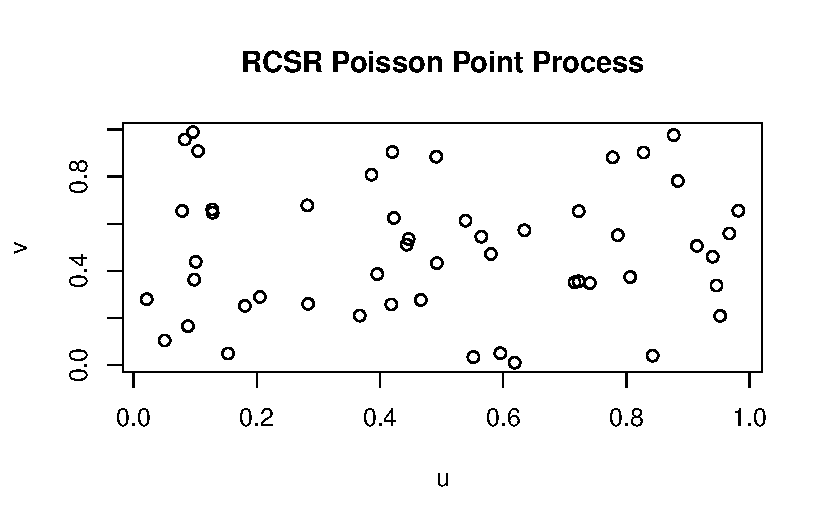
\includegraphics{robby_homework1_files/figure-pdf/unnamed-chunk-7-1.pdf}

}

\end{figure}

\begin{Shaded}
\begin{Highlighting}[]
\NormalTok{point\_count2 }\OtherTok{=} \FunctionTok{length}\NormalTok{(h2}\SpecialCharTok{$}\NormalTok{x)}
\FunctionTok{print}\NormalTok{(}\StringTok{"Total Points Generated: "}\NormalTok{)}
\end{Highlighting}
\end{Shaded}

\begin{verbatim}
[1] "Total Points Generated: "
\end{verbatim}

\begin{Shaded}
\begin{Highlighting}[]
\FunctionTok{print}\NormalTok{(point\_count2)}
\end{Highlighting}
\end{Shaded}

\begin{verbatim}
[1] 51
\end{verbatim}

\hypertarget{problem-8}{%
\subsection{Problem 8}\label{problem-8}}

\begin{quote}
\begin{enumerate}
\def\labelenumi{\arabic{enumi}.}
\tightlist
\item
  Draw a single data set from the rpoispp function. Use the density
  function to estimate the intensity function for the simulated data
  set. Compute the difference between the maximum and minimum estimated
  intensity values.
\end{enumerate}
\end{quote}

\begin{Shaded}
\begin{Highlighting}[]
\NormalTok{dim }\OtherTok{=} \DecValTok{2}
\NormalTok{df }\OtherTok{=} \FunctionTok{rpoispp}\NormalTok{(}\DecValTok{50}\NormalTok{)}
\NormalTok{bx }\OtherTok{=} \FunctionTok{sd}\NormalTok{(df}\SpecialCharTok{$}\NormalTok{x)}\SpecialCharTok{*}\FunctionTok{length}\NormalTok{(df}\SpecialCharTok{$}\NormalTok{x)}\SpecialCharTok{\^{}}\NormalTok{(}\SpecialCharTok{{-}}\DecValTok{1}\SpecialCharTok{/}\NormalTok{(dim}\SpecialCharTok{+}\DecValTok{4}\NormalTok{))}
\NormalTok{by }\OtherTok{=} \FunctionTok{sd}\NormalTok{(df}\SpecialCharTok{$}\NormalTok{y)}\SpecialCharTok{*}\FunctionTok{length}\NormalTok{(df}\SpecialCharTok{$}\NormalTok{y)}\SpecialCharTok{\^{}}\NormalTok{(}\SpecialCharTok{{-}}\DecValTok{1}\SpecialCharTok{/}\NormalTok{(dim}\SpecialCharTok{+}\DecValTok{4}\NormalTok{))}

\NormalTok{ix }\OtherTok{=} \FunctionTok{density}\NormalTok{(df,}\AttributeTok{sigma =} \FunctionTok{c}\NormalTok{(bx,by))}

\NormalTok{ix\_min }\OtherTok{=} \FunctionTok{min}\NormalTok{(ix}\SpecialCharTok{$}\NormalTok{v)}
\NormalTok{ix\_max }\OtherTok{=} \FunctionTok{max}\NormalTok{(ix}\SpecialCharTok{$}\NormalTok{v)}
\NormalTok{ix\_diff\_compare }\OtherTok{=}\NormalTok{ ix\_max }\SpecialCharTok{{-}}\NormalTok{ ix\_min}
\NormalTok{ix\_mean\_compare }\OtherTok{=} \FunctionTok{mean}\NormalTok{(ix}\SpecialCharTok{$}\NormalTok{v)}
\FunctionTok{print}\NormalTok{(ix\_diff\_compare)}
\end{Highlighting}
\end{Shaded}

\begin{verbatim}
[1] 70.47447
\end{verbatim}

\begin{Shaded}
\begin{Highlighting}[]
\FunctionTok{print}\NormalTok{(ix\_mean\_compare)}
\end{Highlighting}
\end{Shaded}

\begin{verbatim}
[1] 64.75937
\end{verbatim}

\begin{Shaded}
\begin{Highlighting}[]
\FunctionTok{plot}\NormalTok{(df}\SpecialCharTok{$}\NormalTok{x,df}\SpecialCharTok{$}\NormalTok{y, }\AttributeTok{xlab =} \StringTok{"u"}\NormalTok{, }\AttributeTok{ylab =} \StringTok{"v"}\NormalTok{,}\AttributeTok{main=}\StringTok{"Poisson Point Process"}\NormalTok{)}
\end{Highlighting}
\end{Shaded}

\begin{figure}[H]

{\centering 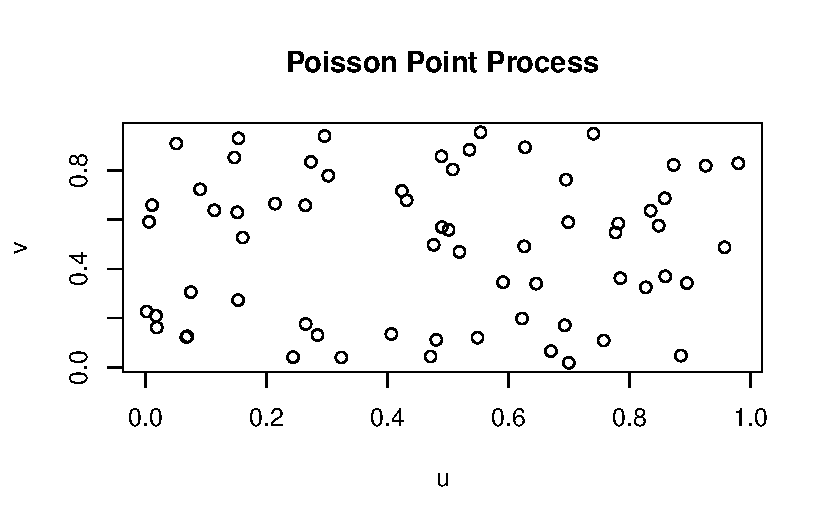
\includegraphics{robby_homework1_files/figure-pdf/unnamed-chunk-9-1.pdf}

}

\end{figure}

\begin{Shaded}
\begin{Highlighting}[]
\NormalTok{point\_count2 }\OtherTok{=} \FunctionTok{length}\NormalTok{(df}\SpecialCharTok{$}\NormalTok{x)}
\FunctionTok{print}\NormalTok{(}\StringTok{"Total Points Generated: "}\NormalTok{)}
\end{Highlighting}
\end{Shaded}

\begin{verbatim}
[1] "Total Points Generated: "
\end{verbatim}

\begin{Shaded}
\begin{Highlighting}[]
\FunctionTok{print}\NormalTok{(point\_count2)}
\end{Highlighting}
\end{Shaded}

\begin{verbatim}
[1] 65
\end{verbatim}

\begin{quote}
\begin{enumerate}
\def\labelenumi{\arabic{enumi}.}
\setcounter{enumi}{1}
\tightlist
\item
  Draw a simulated data set from the `rcsr' function assuming lambda =
  50. Use the density function to estimate the intensity function of the
  simulated data set, and compute the diff between max and min intensity
  values.
\end{enumerate}
\end{quote}

\begin{Shaded}
\begin{Highlighting}[]
\NormalTok{dim }\OtherTok{=} \DecValTok{2}
\NormalTok{lambda }\OtherTok{=} \DecValTok{50}
\NormalTok{df2 }\OtherTok{=} \FunctionTok{rcsr}\NormalTok{(}\DecValTok{50}\NormalTok{)}
\NormalTok{bx }\OtherTok{=} \FunctionTok{sd}\NormalTok{(df2}\SpecialCharTok{$}\NormalTok{x)}\SpecialCharTok{*}\FunctionTok{length}\NormalTok{(df2}\SpecialCharTok{$}\NormalTok{x)}\SpecialCharTok{\^{}}\NormalTok{(}\SpecialCharTok{{-}}\DecValTok{1}\SpecialCharTok{/}\NormalTok{(dim}\SpecialCharTok{+}\DecValTok{4}\NormalTok{))}
\NormalTok{by }\OtherTok{=} \FunctionTok{sd}\NormalTok{(df2}\SpecialCharTok{$}\NormalTok{y)}\SpecialCharTok{*}\FunctionTok{length}\NormalTok{(df2}\SpecialCharTok{$}\NormalTok{y)}\SpecialCharTok{\^{}}\NormalTok{(}\SpecialCharTok{{-}}\DecValTok{1}\SpecialCharTok{/}\NormalTok{(dim}\SpecialCharTok{+}\DecValTok{4}\NormalTok{))}

\NormalTok{ix2 }\OtherTok{=} \FunctionTok{density}\NormalTok{(df2,}\AttributeTok{sigma =} \FunctionTok{c}\NormalTok{(bx,by))}

\NormalTok{ix\_min2 }\OtherTok{=} \FunctionTok{min}\NormalTok{(ix2}\SpecialCharTok{$}\NormalTok{v)}
\NormalTok{ix\_max2 }\OtherTok{=} \FunctionTok{max}\NormalTok{(ix2}\SpecialCharTok{$}\NormalTok{v)}
\NormalTok{ix\_diff2 }\OtherTok{=}\NormalTok{ ix\_max2 }\SpecialCharTok{{-}}\NormalTok{ ix\_min2}
\FunctionTok{print}\NormalTok{(ix\_diff2)}
\end{Highlighting}
\end{Shaded}

\begin{verbatim}
[1] 103.8326
\end{verbatim}

\begin{Shaded}
\begin{Highlighting}[]
\FunctionTok{print}\NormalTok{(}\FunctionTok{mean}\NormalTok{(ix2}\SpecialCharTok{$}\NormalTok{v))}
\end{Highlighting}
\end{Shaded}

\begin{verbatim}
[1] 47.05487
\end{verbatim}

\begin{Shaded}
\begin{Highlighting}[]
\FunctionTok{plot}\NormalTok{(df2}\SpecialCharTok{$}\NormalTok{x,df2}\SpecialCharTok{$}\NormalTok{y, }\AttributeTok{xlab =} \StringTok{"u"}\NormalTok{, }\AttributeTok{ylab =} \StringTok{"v"}\NormalTok{,}\AttributeTok{main=}\StringTok{"RCSR Poisson Point Process"}\NormalTok{)}
\end{Highlighting}
\end{Shaded}

\begin{figure}[H]

{\centering 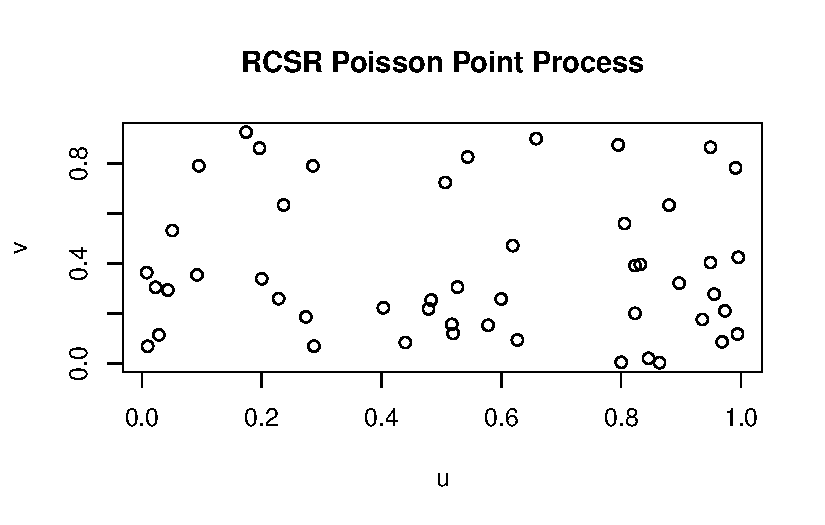
\includegraphics{robby_homework1_files/figure-pdf/unnamed-chunk-11-1.pdf}

}

\end{figure}

\begin{Shaded}
\begin{Highlighting}[]
\NormalTok{point\_count2 }\OtherTok{=} \FunctionTok{length}\NormalTok{(df2}\SpecialCharTok{$}\NormalTok{x)}
\FunctionTok{print}\NormalTok{(}\StringTok{"Total Points Generated: "}\NormalTok{)}
\end{Highlighting}
\end{Shaded}

\begin{verbatim}
[1] "Total Points Generated: "
\end{verbatim}

\begin{Shaded}
\begin{Highlighting}[]
\FunctionTok{print}\NormalTok{(point\_count2)}
\end{Highlighting}
\end{Shaded}

\begin{verbatim}
[1] 49
\end{verbatim}

\begin{quote}
\begin{enumerate}
\def\labelenumi{\arabic{enumi}.}
\setcounter{enumi}{2}
\tightlist
\item
  Repeat previous test 999 times
\end{enumerate}
\end{quote}

\begin{Shaded}
\begin{Highlighting}[]
\NormalTok{dim }\OtherTok{=} \DecValTok{2}
\NormalTok{lambda }\OtherTok{=} \DecValTok{50}
\NormalTok{result }\OtherTok{\textless{}{-}}  \FunctionTok{data.frame}\NormalTok{()}
\NormalTok{diffs }\OtherTok{\textless{}{-}} \FunctionTok{data.frame}\NormalTok{()}

\ControlFlowTok{for}\NormalTok{ (i }\ControlFlowTok{in} \DecValTok{1}\SpecialCharTok{:}\DecValTok{999}\NormalTok{) \{}
\NormalTok{  df }\OtherTok{=} \FunctionTok{rcsr}\NormalTok{(}\DecValTok{50}\NormalTok{)}
\NormalTok{  bx }\OtherTok{=} \FunctionTok{sd}\NormalTok{(df}\SpecialCharTok{$}\NormalTok{x)}\SpecialCharTok{*}\FunctionTok{length}\NormalTok{(df}\SpecialCharTok{$}\NormalTok{x)}\SpecialCharTok{\^{}}\NormalTok{(}\SpecialCharTok{{-}}\DecValTok{1}\SpecialCharTok{/}\NormalTok{(dim}\SpecialCharTok{+}\DecValTok{4}\NormalTok{))}
\NormalTok{  by }\OtherTok{=} \FunctionTok{sd}\NormalTok{(df}\SpecialCharTok{$}\NormalTok{y)}\SpecialCharTok{*}\FunctionTok{length}\NormalTok{(df}\SpecialCharTok{$}\NormalTok{y)}\SpecialCharTok{\^{}}\NormalTok{(}\SpecialCharTok{{-}}\DecValTok{1}\SpecialCharTok{/}\NormalTok{(dim}\SpecialCharTok{+}\DecValTok{4}\NormalTok{))}
  
\NormalTok{  ixr }\OtherTok{=} \FunctionTok{density}\NormalTok{(df,}\AttributeTok{sigma =} \FunctionTok{c}\NormalTok{(bx,by))}
  
\NormalTok{  ix\_minr }\OtherTok{=} \FunctionTok{min}\NormalTok{(ixr}\SpecialCharTok{$}\NormalTok{v)}
\NormalTok{  ix\_maxr }\OtherTok{=} \FunctionTok{max}\NormalTok{(ixr}\SpecialCharTok{$}\NormalTok{v)}
\NormalTok{  ix\_meanr }\OtherTok{=} \FunctionTok{mean}\NormalTok{(ixr}\SpecialCharTok{$}\NormalTok{v)}
\NormalTok{  ix\_diffr }\OtherTok{=}\NormalTok{ ix\_maxr }\SpecialCharTok{{-}}\NormalTok{ ix\_minr}
\NormalTok{  result[i,}\DecValTok{1}\NormalTok{] }\OtherTok{=}\NormalTok{ ix\_meanr}
\NormalTok{  diffs[i,}\DecValTok{1}\NormalTok{] }\OtherTok{=}\NormalTok{ ix\_diffr}
\NormalTok{\}}

\FunctionTok{t.test}\NormalTok{(result,}\AttributeTok{mu=}\NormalTok{ix\_mean\_compare)}
\end{Highlighting}
\end{Shaded}

\begin{verbatim}

    One Sample t-test

data:  result
t = -61.505, df = 998, p-value < 2.2e-16
alternative hypothesis: true mean is not equal to 64.75937
95 percent confidence interval:
 49.84064 50.76319
sample estimates:
mean of x 
 50.30192 
\end{verbatim}

\begin{quote}
The p-value of the RCSR generated data indicates that we should reject
the null hypothesis that the intensities from the RCSR data set are
statistically equivalent to the rpois data set. This in turn implies
that the RCSR dataset fails to produce a point process that could be
classified as CSR. This could be because the rpois data set will have a
mean anywhere within the range of a poisson distribution with parameter
lambda equal to 50, sometimes above or below 50 by enough to show a
statistical difference between the observed means.
\end{quote}

\hypertarget{problem-9}{%
\subsection{Problem 9}\label{problem-9}}

\begin{Shaded}
\begin{Highlighting}[]
\NormalTok{numata\_pines }\OtherTok{\textless{}{-}}\NormalTok{ spatstat.data}\SpecialCharTok{::}\NormalTok{japanesepines}
\FunctionTok{plot}\NormalTok{(numata\_pines}\SpecialCharTok{$}\NormalTok{x,numata\_pines}\SpecialCharTok{$}\NormalTok{y,}\AttributeTok{xlab=}\StringTok{\textquotesingle{}U\textquotesingle{}}\NormalTok{,}\AttributeTok{ylab=}\StringTok{\textquotesingle{}V\textquotesingle{}}\NormalTok{,}\AttributeTok{main=}\StringTok{\textquotesingle{}Japanese Black Pine Sapling Locations\textquotesingle{}}\NormalTok{)}
\end{Highlighting}
\end{Shaded}

\begin{figure}[H]

{\centering 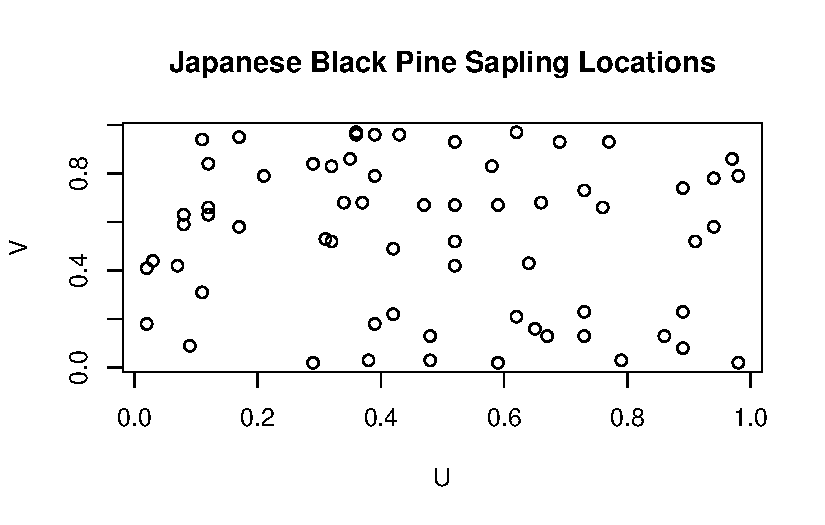
\includegraphics{robby_homework1_files/figure-pdf/unnamed-chunk-13-1.pdf}

}

\end{figure}

\begin{Shaded}
\begin{Highlighting}[]
\NormalTok{bx }\OtherTok{=} \FunctionTok{sd}\NormalTok{(numata\_pines}\SpecialCharTok{$}\NormalTok{x)}\SpecialCharTok{*}\FunctionTok{length}\NormalTok{(numata\_pines}\SpecialCharTok{$}\NormalTok{x)}\SpecialCharTok{\^{}}\NormalTok{(}\SpecialCharTok{{-}}\DecValTok{1}\SpecialCharTok{/}\NormalTok{(dim}\SpecialCharTok{+}\DecValTok{4}\NormalTok{))}
\NormalTok{by }\OtherTok{=} \FunctionTok{sd}\NormalTok{(numata\_pines}\SpecialCharTok{$}\NormalTok{y)}\SpecialCharTok{*}\FunctionTok{length}\NormalTok{(numata\_pines}\SpecialCharTok{$}\NormalTok{y)}\SpecialCharTok{\^{}}\NormalTok{(}\SpecialCharTok{{-}}\DecValTok{1}\SpecialCharTok{/}\NormalTok{(dim}\SpecialCharTok{+}\DecValTok{4}\NormalTok{))}

\NormalTok{ix }\OtherTok{=} \FunctionTok{density}\NormalTok{(numata\_pines,}\AttributeTok{sigma =} \FunctionTok{c}\NormalTok{(bx,by))}
\FunctionTok{contour}\NormalTok{(ix}\SpecialCharTok{$}\NormalTok{v,}\AttributeTok{main=}\StringTok{\textquotesingle{}Japanese Black Pine Sapling Contours\textquotesingle{}}\NormalTok{)}
\end{Highlighting}
\end{Shaded}

\begin{figure}[H]

{\centering 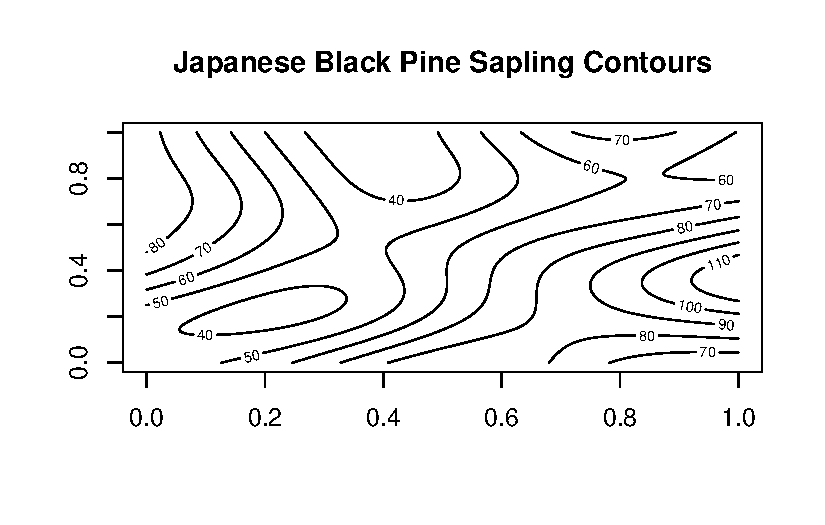
\includegraphics{robby_homework1_files/figure-pdf/unnamed-chunk-14-1.pdf}

}

\end{figure}

\begin{quote}
The observed data appears to be compatible with CSR as the intensity
varies and no obvious clustering can be seen, though some overlapping
event locations imply the points are not regular either.
\end{quote}



\end{document}
